\documentclass{article}
\usepackage[margin=1in]{geometry}
\usepackage{amsmath,amssymb}
\usepackage{verbatim}
\usepackage{graphicx}
\usepackage{xcolor,colortbl}
\usepackage[]{algorithm2e}
\usepackage{cite}
\usepackage{caption}
\usepackage{mdframed}

%\usepackage{soul}

\newcommand{\tab}{\hspace{10mm}}
\newcommand{\dtab}{\hspace{20mm}}
\newcommand{\ttab}{\hspace{30mm}}
\newcommand{\qtab}{\hspace{40mm}}

\begin{document}

\title{Autonomous Agents 1 \\ Assignment 2}

\author{By Group 4: Gieske, Gornishka, Koster, Loor}
\maketitle

\pagebreak

\section*{Introduction}
This report contains the analysis of an implementation of single agent reinforcement learning. In these algorithms, the agent has no prior knowledge of the transition or reward function. Two different solutions to this problem are presented: in model-based learning, the agent learns the model from experience and plans on the learned model. In model-free learning, the agent learns state-values or Q-values directly. In this paper, model-free learning methods are considered.\\
Some prominent model-free reinforcement learning methods are on- and off-policy Monte Carlo, Q-learning (off-policy) and Sarsa (on-policy), where on-policy methods evaluate the values of a policy $\pi$ \textit{as it's being followed}, while off-policy methods allow the agent to follow a different policy $\pi'$. This paper reports on Q-learning and its on-policy equivalent, Sarsa. Moreover, the difference in action-selection between $\epsilon$-greedy and softmax are compared. 
\pagebreak

\section*{Theory}
\subsection*{Temporal difference learning methods}
Temporal difference learning methods estimate state-values or Q-values by updating them on every time step (as opposed to the episodic updates of Monte Carlo-methods).
Temporal difference learning methods are similar to Monte Carlo methods in that they both learn from experience directly, without requiring a model (thus, they do not exploit the Bellman-equations in equations \ref{eq:bellmanV} and \ref{eq:bellmanQ}) and they are similar to dynamic programming methods in that they both \textit{bootstrap}, i.e. they estimate values based on earlier estimates. 
\begin{mdframed}
\begin{align}
V^*(s) &= \sum_{s'} \mathcal{P}^a_{ss'}\left[ \mathcal{R}^a_{ss'} + \gamma \underset{a}{\text{max}}V^*(s') \right]\label{eq:bellmanV}\\
Q^*(s,a) &= \sum_{s'} \mathcal{P}^a_{ss'}\left[ \mathcal{R}^a_{ss'} + \gamma \underset{a}{\text{max}}Q^*(s', a') \right]\label{eq:bellmanQ}
\end{align}
\end{mdframed}

Thus, in general, an update-rule for a TD-method would be similar to that of TD(0) in equation \ref{eq:td0}.
\begin{mdframed}
\begin{align}
V(s) \leftarrow V(s) + \alpha [r+\gamma V(s') - V(s)]\label{eq:td0}
\end{align}
\end{mdframed}
Both Q-learning and Sarsa are TD-methods, and are described in more detail in sections Q-learning and Sarsa.

\subsection*{Q-Learning} 
Q-learning is a temporal difference method that uses\footnote{More specifically, this is \textit{one-step Q-learning}, which is the algorithm evaluated in this paper.} the update rule in equation \ref{eq:qupdate}. Because it retrieves the Q-value of the state-action pair where Q(s', a) is maximized, it is an \textit{off-policy} method. The algorithm for Q-learning can be found in pseudocode in figure \ref{alg:qlearning}.

\begin{mdframed}
\begin{align}
Q(s_t, a_t) \leftarrow Q(s_t,a_t) + \alpha \left[ r_{t+1} + \gamma \underset{a}{\text{max}} Q(s_{t+1},a) - Q(s_t,a_t)\right]\label{eq:qupdate}
\end{align}
\end{mdframed}


\begin{figure}[h!] 
\begin{mdframed}
\begin{algorithm}[H]
Initialize Q(s,a) arbitrarily \\
Repeat (for each episode):\\
\tab Initialize s \\
\tab Repeat (for each step of episode):\\
\dtab Choose a from s' using policy derived from Q (e.g., $\epsilon$-greedy)\\
\dtab Take action a, observe r, s'\\
\dtab Q(s,a) $\leftarrow$ Q(s,a) + $\alpha [ r + \gamma \max_a' Q(s', a') - Q(s, a) ]$  \\
\dtab s $\leftarrow$ s'; \\
\tab until s is terminal\\
\end{algorithm}
\end{mdframed}
\caption{The algorithm for one-step Q-learning\cite{bartosutton}}
\label{alg:qlearning}
\end{figure}



\subsection*{Sarsa}
Sarsa is a temporal difference method that uses the update rule in equation \ref{eq:sarsaupdate}. Because it retrieves the Q-value of the state-action pair (s', a') where a' is selected using the policy $\pi$ that is being evaluated, it is an \textit{on-policy} method. The algorithm for Sarsa can be found in pseudocode in figure \ref{alg:sarsa}.
\begin{mdframed}
\begin{align}
Q(s_t, a_t) \leftarrow Q(s_t,a_t) + \alpha \left[ r_{t+1} + \gamma Q(s_{t+1},a_{t+1}) - Q(s_t,a_t)\right]\label{eq:sarsaupdate}
\end{align}
\end{mdframed}


\begin{figure}[h!]
\begin{mdframed}
\begin{algorithm}[H]
Initialize Q(s,a) arbitrarily\\
Repeat (for each episode):\\
\tab Initialize s \\
\tab Choose a from s' using policy derived from Q (e.g., $\epsilon$-greedy)\\
\tab Repeat (for each step of episode):\\
\dtab Take action a, observe r, s'\\
\dtab Choose a' from s' using policy derived from Q (e.g., $\epsilon$-greedy)\\
\dtab Q(s,a) $\leftarrow$ Q(s,a) + $\alpha [ r + \gamma Q(s', a') - Q(s, a) ]$ \\
\dtab s $\leftarrow$ s'; \\
\tab until s is terminal\\
\end{algorithm}
\end{mdframed}
\caption{The algorithm for Sarsa \cite{bartosutton}}
\label{alg:sarsa}
\end{figure}



\subsection*{Monte Carlo Methods}
As stated before, there are several ways of learning a estimating value functions and discovering optimal policies. Again, Monte Carlo methods do not know (nor need) complete knowledge of the environment. Monte Carlo methods require only experience, such as sample sequences of states, actions, and rewards, from on-line interaction with an environment. Unlike TD-methods, Monte Carlo methods require a model. The model only needs to generate sample transitions, unlike Dynamic Programming methods which need complete probability distributions of all possible transitions. Therefore, Monte Carlo methods are an important tool for an agent to use when only the model is known.

\subsection*{On-policy Monte Carlo Control}
On-policy Monte Carlo control (OPMCC) does not use exploring starts. In order to ensure that each state is visited and each action is selected infinitely often is to keep selecting these actions. There are two ways of implementing OPMCC; first-visit Monte Carlo and every-visit Monte Carlo. In this case, every-visit Monte Carlo is implemented which is reflected in the algorithm below. 

 
\begin{figure}[h!]
\begin{mdframed}
\begin{algorithm}[H]
Initialize, for all $s \in \mathcal(S), a \in \mathcal(A)(s)$\\
Repeat forever:\\
\tab Generate an episode using exploring starts and $\pi$\\
\tab For each pair s,a appearing in the episode:\\
\dtab $\mathcal{R} \leftarrow $ return following the first occurence of s,a\\
\ttab Append $\mathcal{R}$ to $Returns(s,a)$\\
\ttab $Q(s,a) \leftarrow$ average($Returns(s,a)$)\\
\dtab For each $s$ in the episode:\\
\ttab $a^* \leftarrow$ arg $\max\limits_a Q(s,a)$\\
\ttab For all $a \in \mathcal{A}(s)$:\\

\qtab \[\pi(s,a) \leftarrow \left \{
\begin{array}{l l}
1-\epsilon + \dfrac{\epsilon}{|\mathcal{A}(s)|} & \quad \textit{if } a = a^* \\
\dfrac{\epsilon}{|\mathcal{A}(s)|} & \quad \textit{if } a \neq a^*
\end{array}\right.\]
\end{algorithm}
\end{mdframed}
\caption{The algorithm for on-policy Monte Carlo \cite{bartosutton}}
\label{alg:OPMCC}
\end{figure}





\subsection*{Action selection methods}
In order to select which action to choose according to a given policy, a tradeoff between exploration and exploitation must take place. This tradeoff is important when performing reinforcement learning as the rewards must be maximized, but exploration may lead to finding higher rewards. There are several action selection methods which can be used to select actions. The two techniques analyzed in this report are $\epsilon$-greedy and softmax action selection.

In the case of $\epsilon$-greedy, the best action $a^*$ is given a probability of $1-\epsilon$. All actions $a$ (including $a^*$) then receive an equal portion of $\epsilon$ as a probability. This is formalized in equation \ref{eq:greedy}.
\begin{mdframed}
\begin{align}
\forall a \in \mathcal{A}:p(a) = 
\begin{cases}\label{eq:greedy}
	1 - \epsilon + \frac{\epsilon}{|\mathcal{A}|}, & \text{if } a = a^*\\
	\frac{\epsilon}{|\mathcal{A}|} & \text{otherwise }
\end{cases}
\end{align}
\end{mdframed}
So that in $1-\epsilon$ of the cases, $a^*$ is selected, and in $\epsilon$ of the cases a random action is chosen uniformly. Thus, an $\epsilon$-greedy policy mainly exploits the known states to maximize the immediate reward. At probabilistically determined times however, this policy will explore new states. This may lead to undesired behavior as it is possible for the agent to stand beside the goal state when the $\epsilon$-greedy policy turns to explore a new state, which can lead to high negative rewards in particular cases, such as a robot falling off a cliff. Also, $\epsilon$-greedy does not consider the quality of non-optimal actions: an action with a value just below that of $a^*$ receives the same probability as an action with a much lower value. Another note using $\epsilon$-greedy is the intuition that $\epsilon$ should decay as the agent has explored more states, as exploration is adding less information over time. There is, however, no clear-cut way to do decide how and when to decay $\epsilon$.

Softmax action-selection offers a solution to one problem presented by $\epsilon$-greedy policies. The greedy action $a^*$ is still assigned the highest probability, but all other probabilities are ranked and weighted according to their values [1]. There are several ways of implementing the softmax action selection method, but for the purposes of this paper softmax uses a Boltzmann distribution, formalized in \ref{eq:softmax}.
\begin{mdframed}
\begin{align}
\forall a: p_t(a) &= \frac{\text{e}^{Q_t(a)/\tau}}{\sum^n_{b=1}\text{e}^{Q_t(b)/\tau}} \label{eq:softmax}
\end{align}
\end{mdframed}
The parameter $\tau$ in equation $(2)$ is the \textit{temperature} of the distribution. Low temperatures cause the values of $Q_t(a)$ and consequently those of e$^{Q_t(a)/\tau}$ to grow very larger, thus increasing their differences. For high temperatures, the opposite is true, where in the limit $\tau\rightarrow0$, all actions become equiprobable [1].

It is unclear whether $\epsilon$-greedy action selection is better than softmax action selection. The performance of either method may depend on the task at hand and human factors. Experimenting with both methods will lead to more insight in both algorithms.
\pagebreak

\section*{Implementation}
The implementation consists of the following files:
\begin{description}
	\item[Agents\_new] \hfill \\ 
	This file contains implementions of the Agent class, the Prey class and the Predator class. Both the predator and the prey inherit functions of the Agent class. The Agent class contains functions any agent needs, such as a set of actions, a policy and other functions. As the predator is the agent is the agent this implementation focuses on, the predator class contains more functions than the predator class.
	
	\item[Helpers] \hfill \\ 
	This file contains many helper functions. These functions aid in computation and decision making, but cannot (and need not) be part of a specific class.
	
	\item[Other\_objects] \hfill \\ % uncertain about policy class description
	This file contains the Policy and Environment classes. The environment of the game as well as the rules are implemented in the Environment class. The Policy class contains the implementation of Q-Learning, Sarsa, $\epsilon$-greedy, softmax action selection and more functions that help in determining and optimizing a policy as well as choosing an action of this policy.
	\item[Newstate] \hfill \\ 
	This file contains the Game class as well as a demonstration function. The Game class instantiates the game, initialized the predator and the prey and assigns policies to these. The game is run N times and the result is printed. The demonstration function also performs Q-Learning, Sarsa and Monte Carlo. It also uses $\epsilon$-greedy and softmax action selection. The results are printed in the command line and graphs are used for analyzation.
\end{description}
\pagebreak
\section*{Analysis}
This section discusses the results of the implementations.
\subsection*{Q-Learning}
First, let's have a look at the effect of different discount factors on Q-learning. This is displayed in the figure below.

\begin{figure}[h!]
\begin{center}

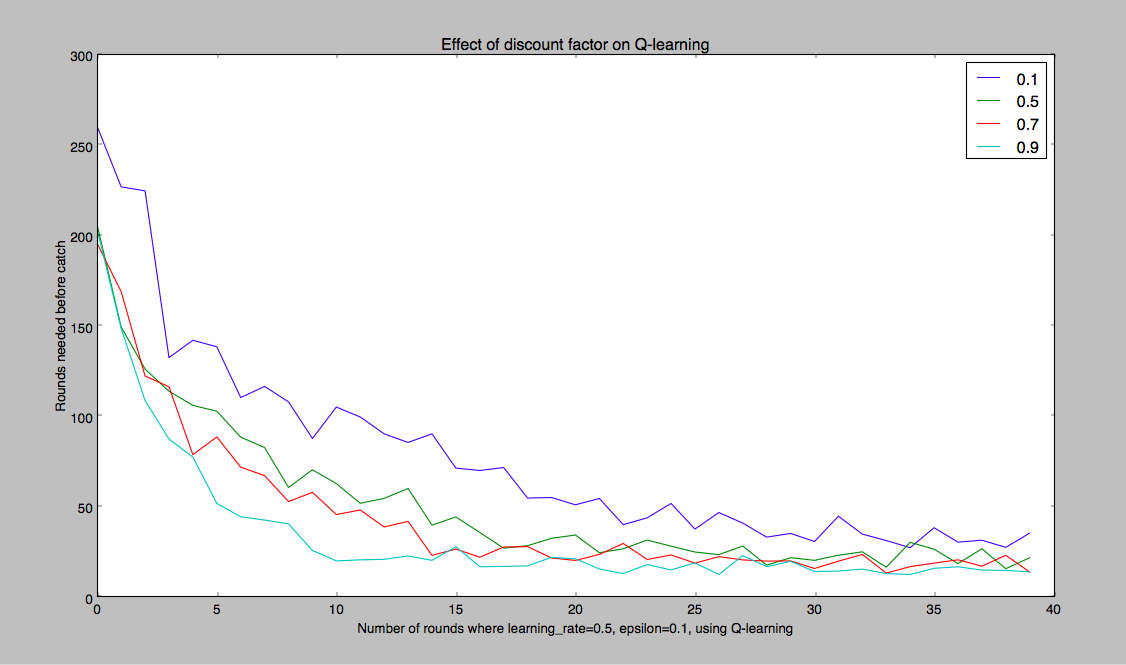
\includegraphics[scale=0.4]{discount_factors}
\caption{Q-learning using different discount factors}
\end{center}

\end{figure}

As shown, the higher the discount factor, the better the result. The height of the discount factor determines the importance of future rewards. A low discount rate tries to achieve a high immediate reward and a high discount rate tries to achieve a high overall reward. Since reaching each state yields a reward of 0, except for the goal state which yields a reward of 10, the future reward must be maximized. Therefore, this behaviour can be expected. 
\\
\\

Now let's analyse the effect of epsilon in the $\epsilon$-greedy algorithm. 

\begin{center}
	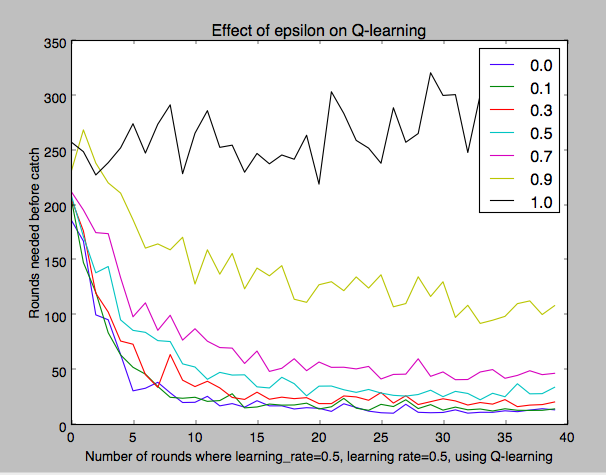
\includegraphics[scale=0.4]{epsilons}
	\captionof{figure}{Q-learning using different epsilon values}
\end{center}



As shown in the figure above, the lower the $\epsilon$ value is, the quicker the algorithm finds the optimal path. This can be expected since, as stated in the theory, an $\epsilon$ value of 0 leads to a greedy algorithm. What is interesting is that an $\epsilon$ value of 0.9 performs quite well compared to a completely exploratory policy, which seems to lead to completely random results. This shows how strong an $\epsilon$-greedy policy is. Even with the slightest bit of greedy behaviour, good results will be achieved.



Now let's analyse the effect of learning rates. 

\begin{center}
	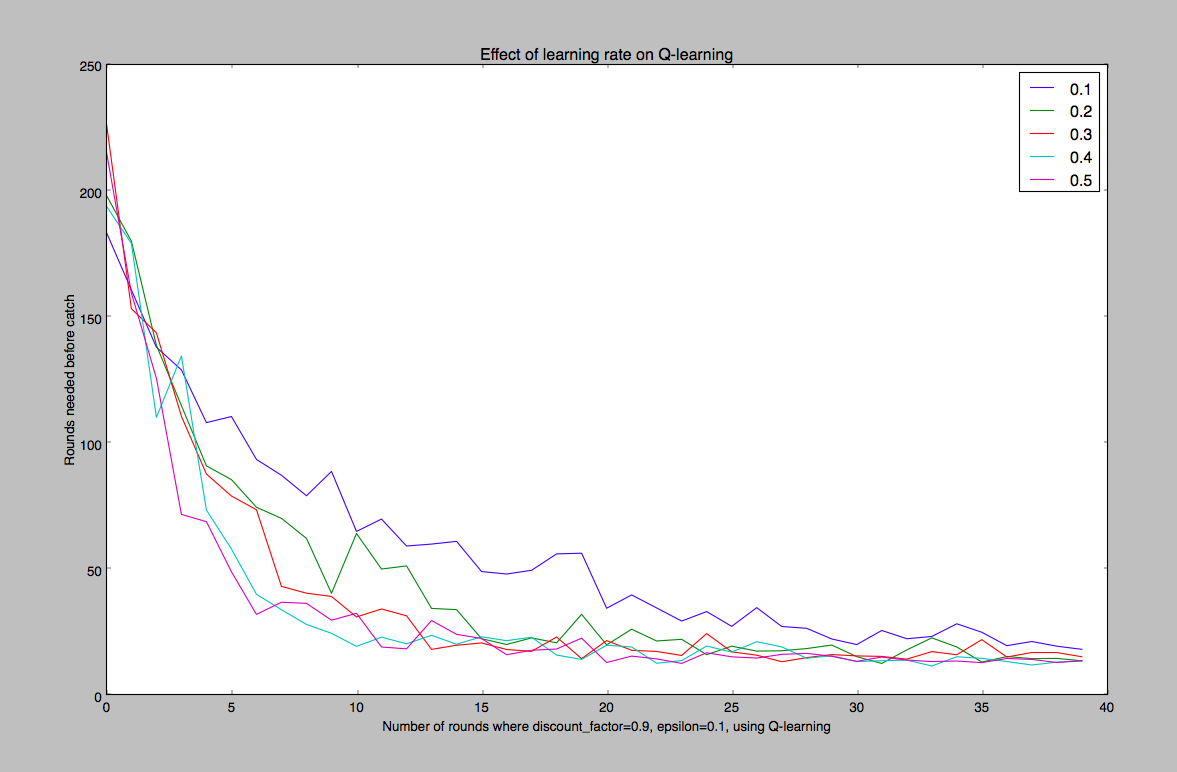
\includegraphics[scale=0.4]{learning_rates}
	\captionof{figure}{Q-learning using different learning rates}
\end{center}

%\begin{figure}[h]
%\begin{center}

%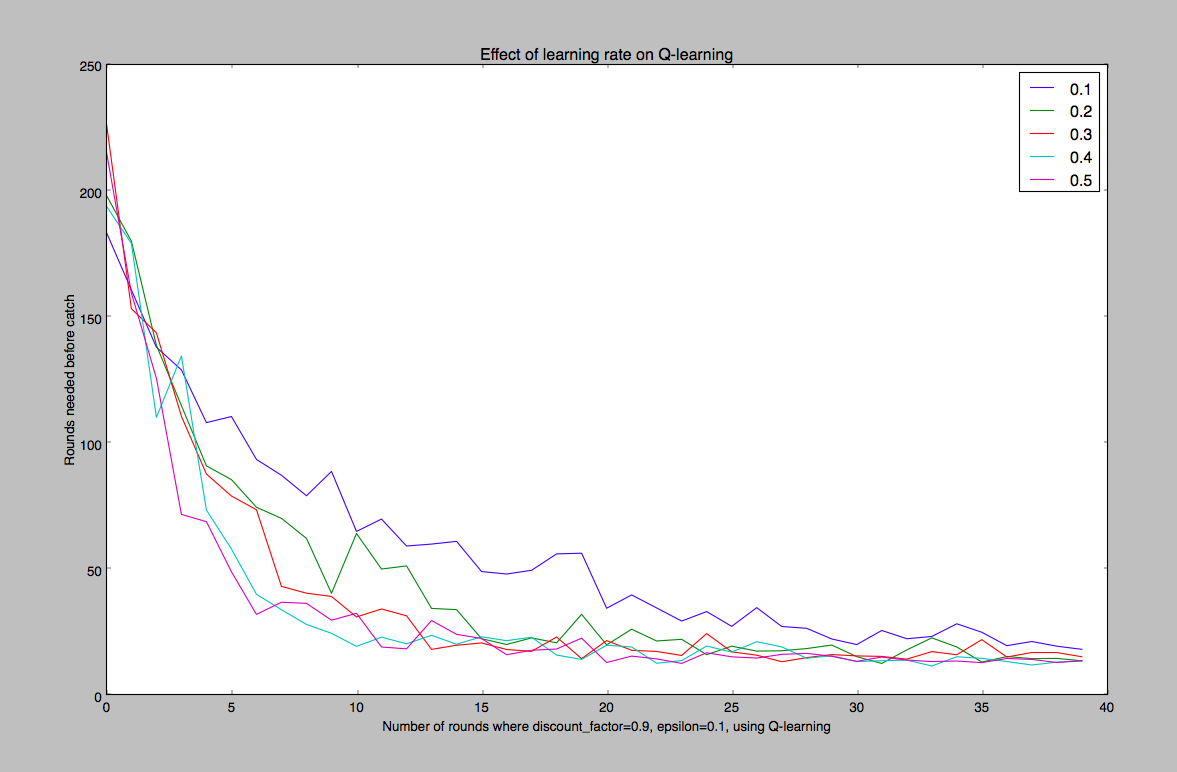
\includegraphics[scale=0.4]{learning_rates}
%\caption{Q-learning using different learning rates}
%\end{center}
%\end{figure}

The figure above shows that for each learning rate between, and including, 0.1 and 0.5 leads to conversion. However, a low conversion rate leads to slower conversion than a high conversion rate. It is interesting to note that the learning rates of both 0.4 and 0.5 appear to converge at about the same speed. The learning rate determines to which extent the new information will overwrite the old information. It appears that, even when storing little new data, this leads to convergence. The more new data overwrites the old data the quicker the algorithm converges. This seems to be correct. However, overwriting all old data might lead to less than optimal behaviour. As stated before, learning rates of 0.4 and 0.5 seem to yield the same result. It is well possible that this is the limit until which the learning rate factor is beneficial to the algorithm. As this lies beyond the scope of this analysis, this can be researched in the future.

\subsection*{Learning types}
Aside from Q-learning, Sarsa and on-policy Monte Carlo were implemented. The results are shown in the figure below.

\begin{center}
	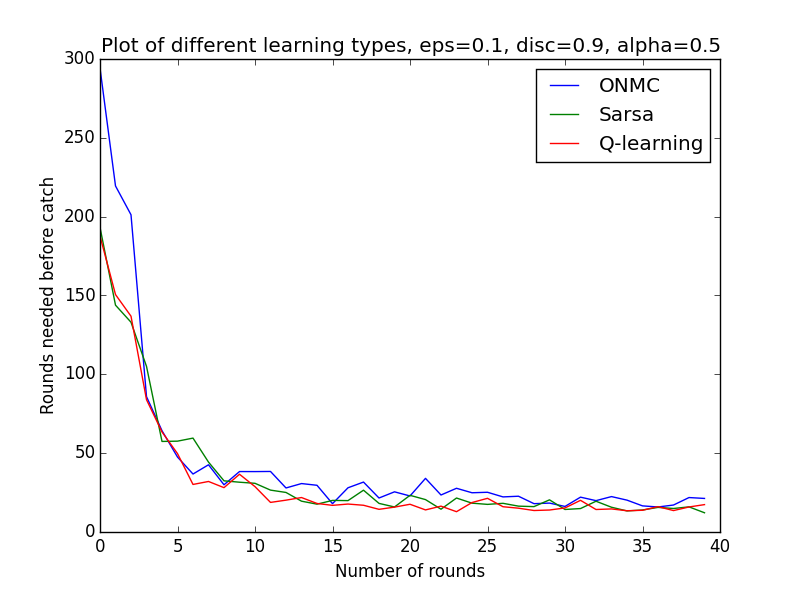
\includegraphics[scale=0.4]{learning_types}
	\captionof{figure}{Different learning types set out against one another}
\end{center}

%\begin{figure}[h]
%\begin{center}

%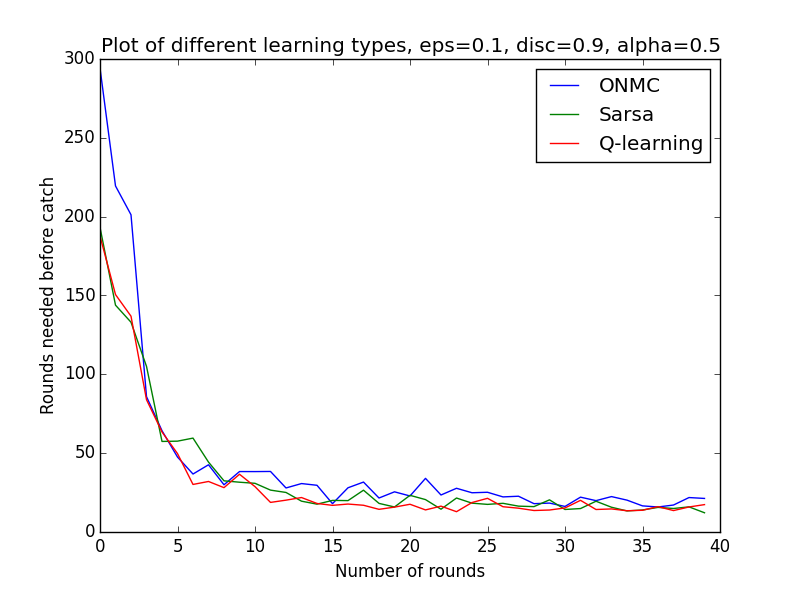
\includegraphics[scale=0.4]{learning_types}
%\caption{Different learning types set out against one another}
%\end{center}
%\end{figure}
The figure shows that all algorithms converge. Q-learning and Sarsa both converge with almost the same speed. On-policy Monte Carlo also converges quickly, but it starts with the worst Q-values. It also shows that of all algorithms, on-policy Monte Carlo performs worst. %explain why
%\subsection*{Sarsa}
\subsection*{$\epsilon$-greedy vs. softmax}
As the effect of $\epsilon$-greedy action selection on Q-learning has already been discussed, let's analyse the effect of softmax action value selection. 
% Explain that smaller grid takes longer to converge, since the predator is more likely to catch the prey, so it takes more rounds to actually explore enough. On the other hand, in a bigger grid the predator is highly unlikely to catch the prey, so it would explore a lot even in one round by the time it catches the prey.

\begin{center}
	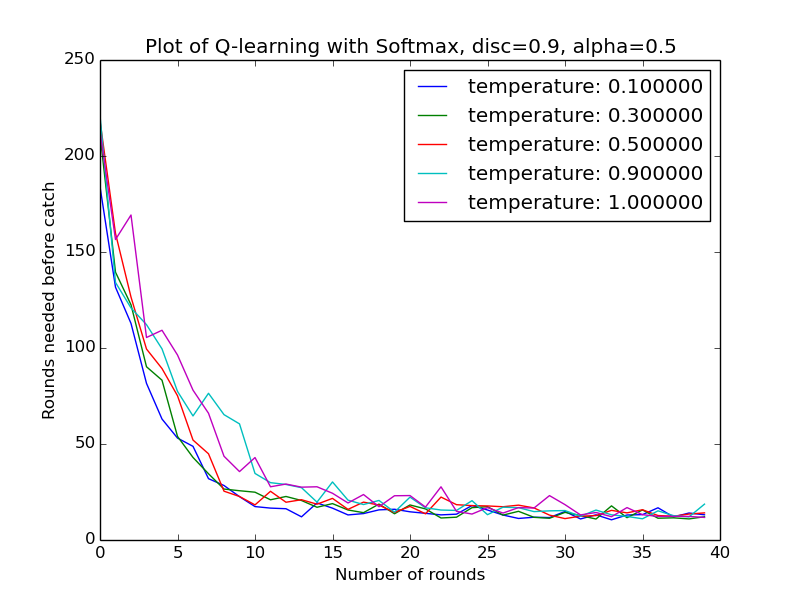
\includegraphics[scale=0.4]{softmax_with_legend}
	\captionof{figure}{Q-learning using different temperatures in Soft-max}
\end{center}

%\begin{figure}[h]
%\begin{center}

%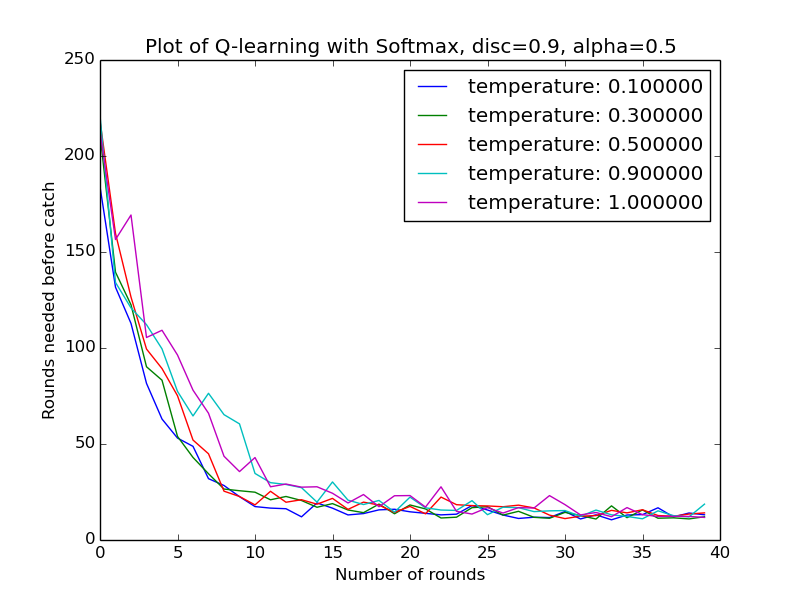
\includegraphics[scale=0.4]{softmax_with_legend}
%\caption{Q-learning using different temperatures in Soft-max}
%\end{center}

%\end{figure}
Now let's look at the results between softmax and $\epsilon$-greedy. As stated in the theory, the difference in effect between softmax action selection and $\epsilon$-greedy action selection is unknown. The performance of either relies on the goal of the implementation, as well as human factors. Therefore, it is imperative to research the effects on this implementation.

\begin{center}
	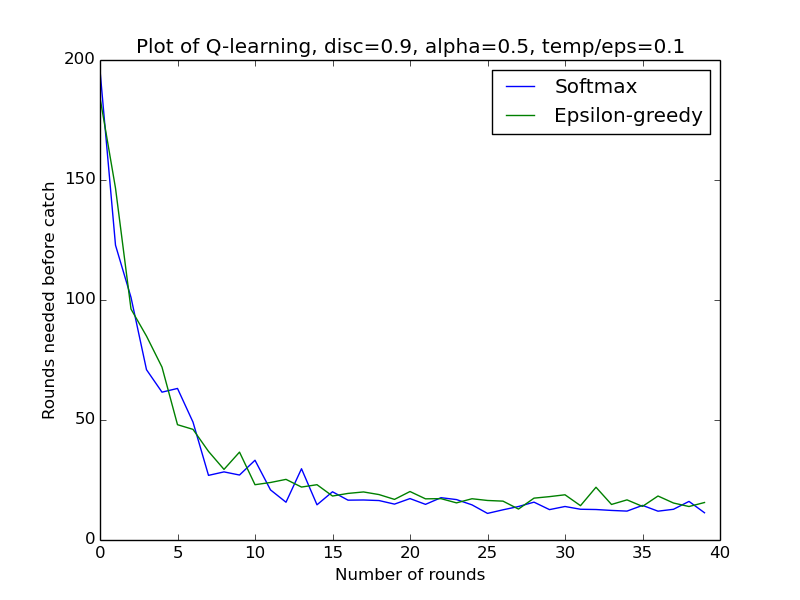
\includegraphics[scale=0.4]{softmax_vs_egreedy}
	\captionof{figure}{Q-learning $\epsilon$-greedy and softmax action selection}
\end{center}
%\begin{figure}[h]
%\begin{center}

%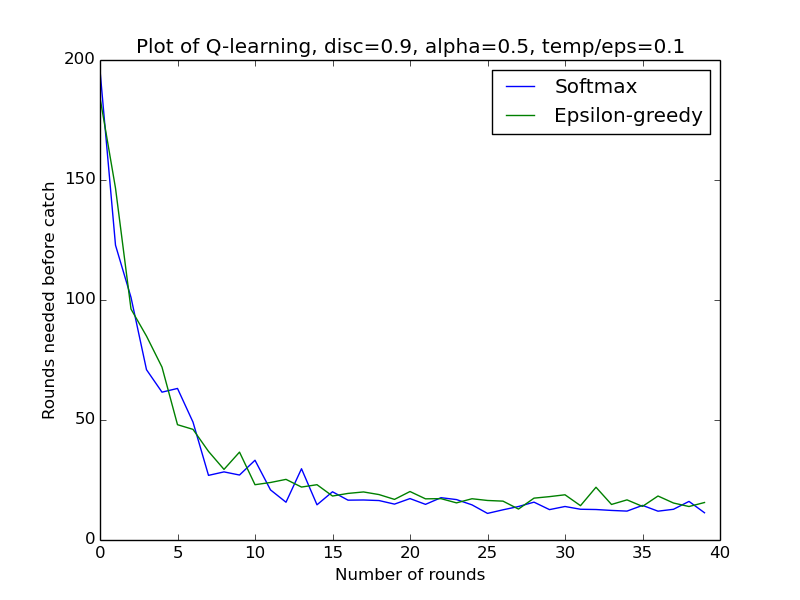
\includegraphics[scale=0.4]{softmax_vs_egreedy}
%\caption{Q-learning $\epsilon$-greedy and softmax action selection}
%\end{center}

%\end{figure}
The figure shows that both softmax and $\epsilon$-greedy action selection yield similar results. Therefore, either can be used. 
\subsection*{Effect of discount rates on learning}
\subsubsection*{Q-learning}
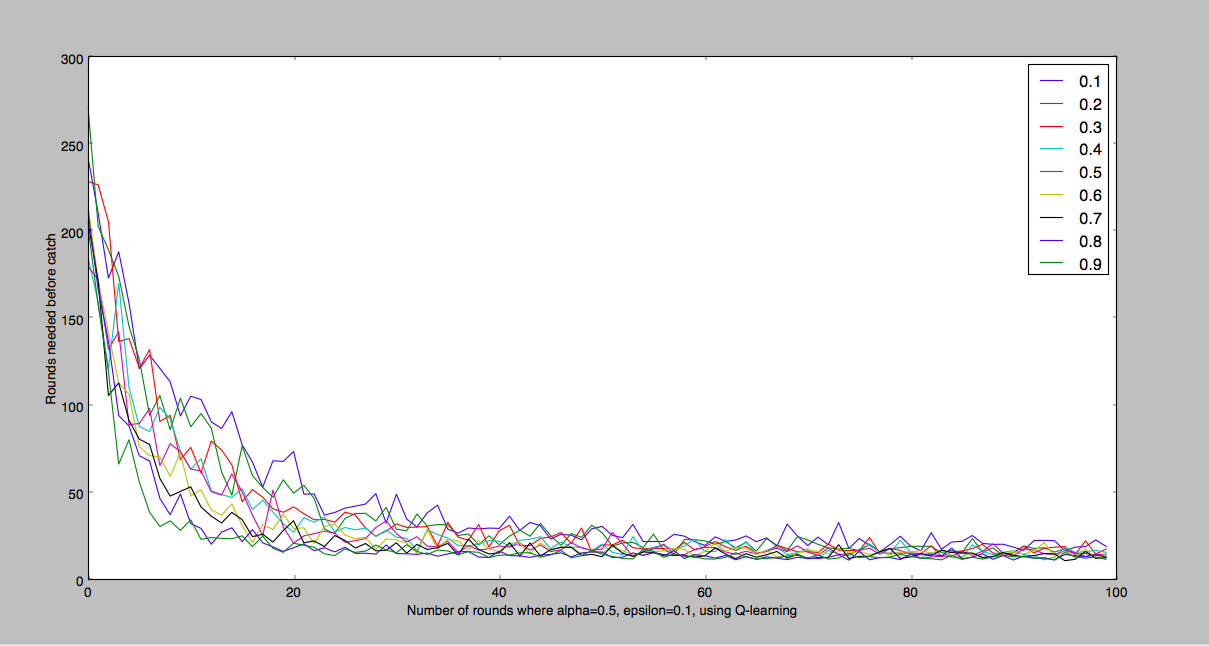
\includegraphics[scale=0.25]{discount_rates_qlearning}
\subsection*{Different initialization for Q-learning}
It was advised to initialize the grid optimistically, when performing Q-learning. When initializing a grid optimistically, it is interesting to see what happens when a grid is not optimistically initialized. The values chosen are 15, 10, 5, 0 and -5. To see the effect of learning, the $\epsilon$-value was either 0 or 0.1. The figure below shows the results of $\epsilon$ value 0.1.

\begin{center}
	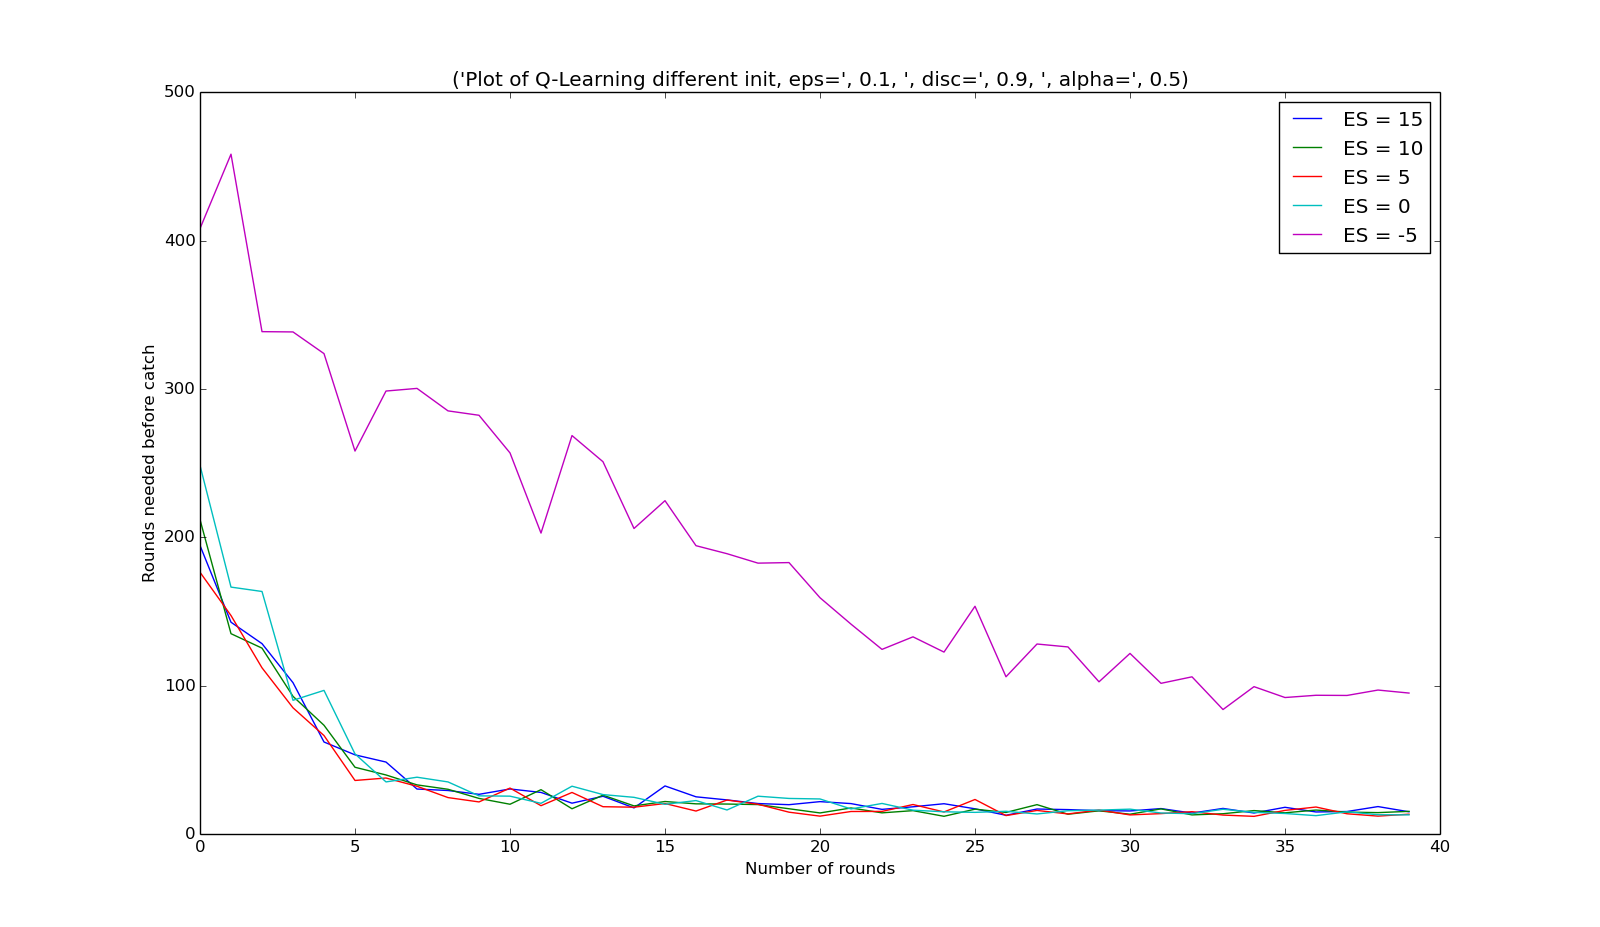
\includegraphics[scale=0.4]{q_learnin_diff_init_epsilon_0_1}
	\captionof{figure}{Q-learning with different initialization values and $\epsilon$ is 0.1}
\end{center}

%\begin{figure}[h]
%\begin{center}
%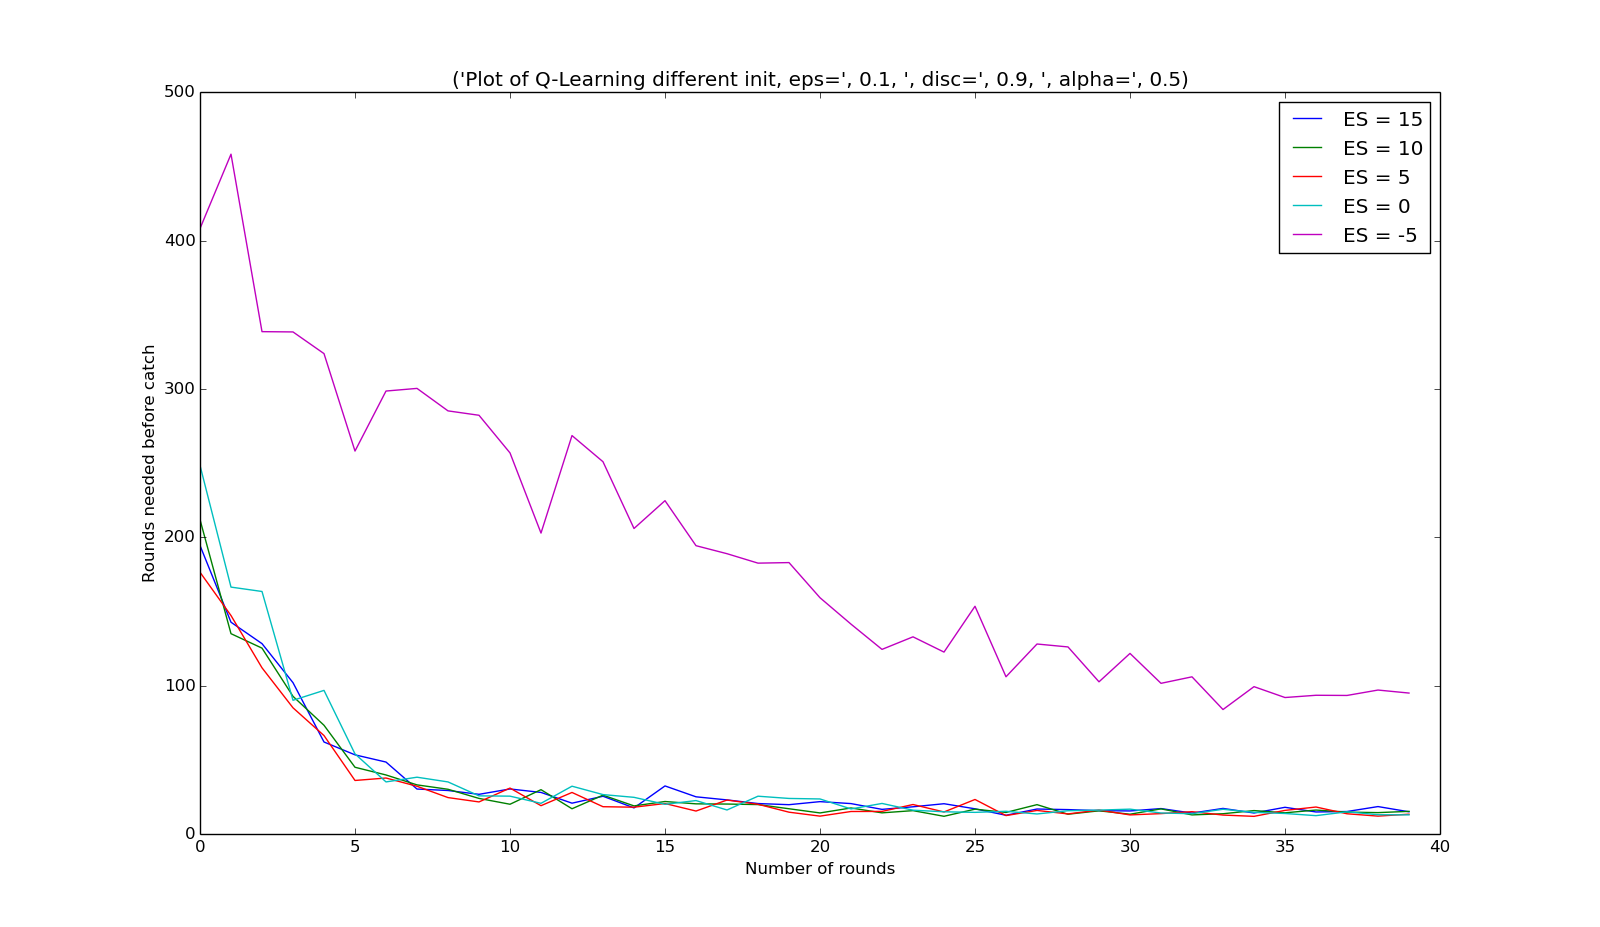
\includegraphics[scale=0.4]{q_learnin_diff_init_epsilon_0_1}
%\caption{Q-learning with different initialization values and $\epsilon$ is 0.1}
%\end{center}
%\end{figure}

Now let's analyse the same initialization values with an $\epsilon$-value of 0.
\begin{center}
	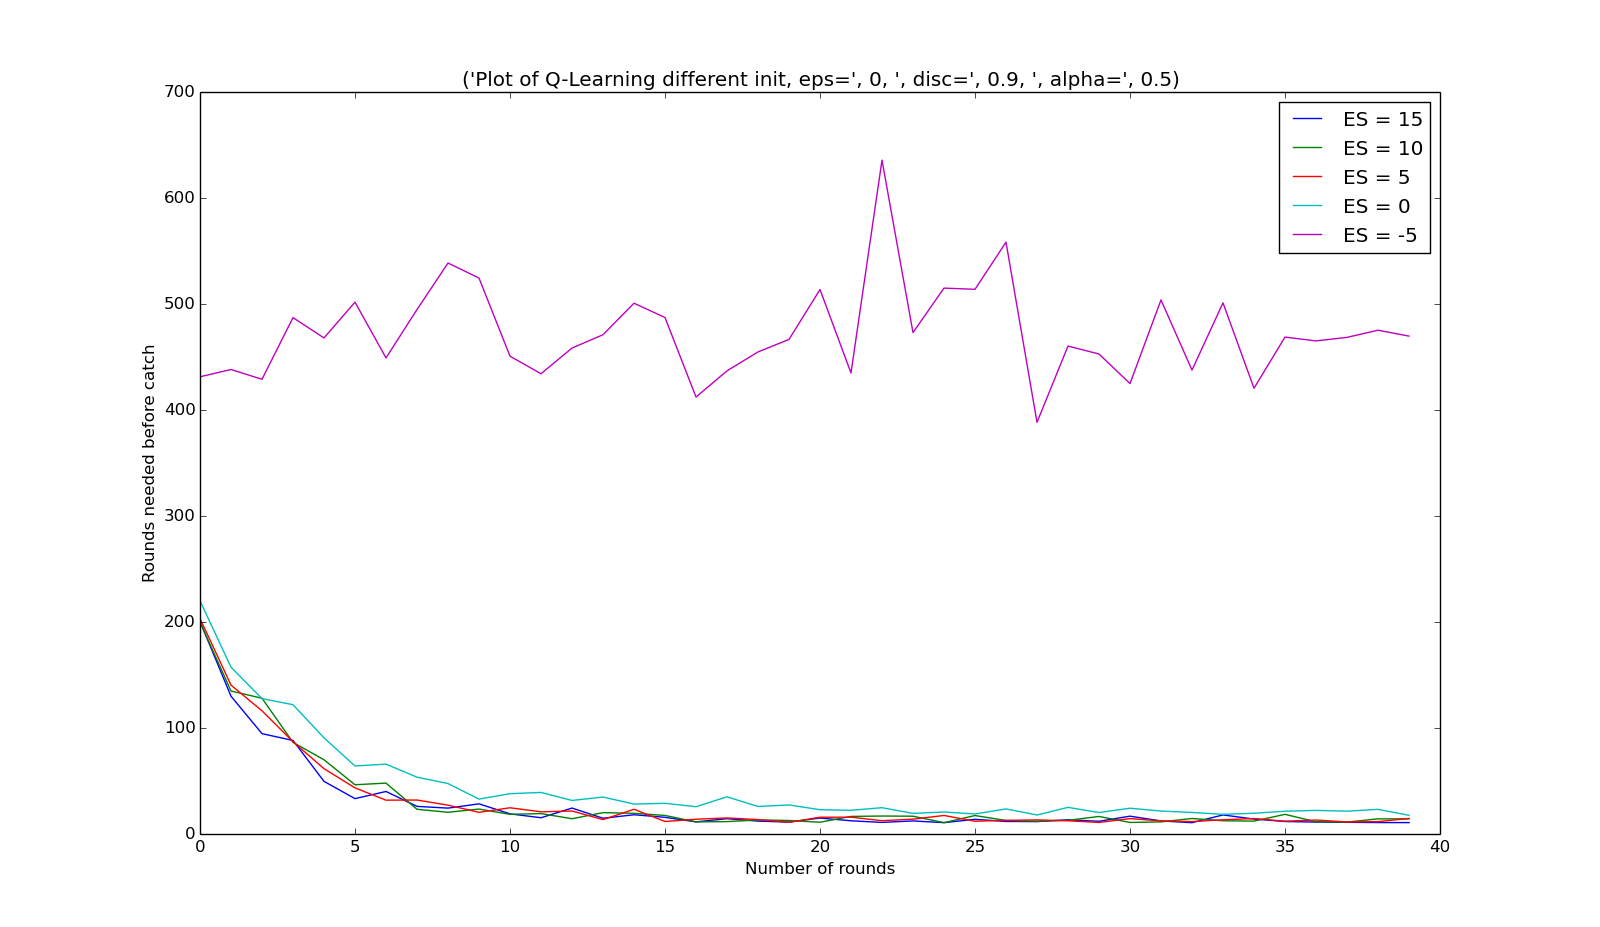
\includegraphics[scale=0.4]{q_learning_diff_init_epsilon_0}
	\captionof{figure}{Q-learning with different initialization values and $\epsilon$ is 0}
\end{center}

%\begin{figure}[h]
%\begin{center}
%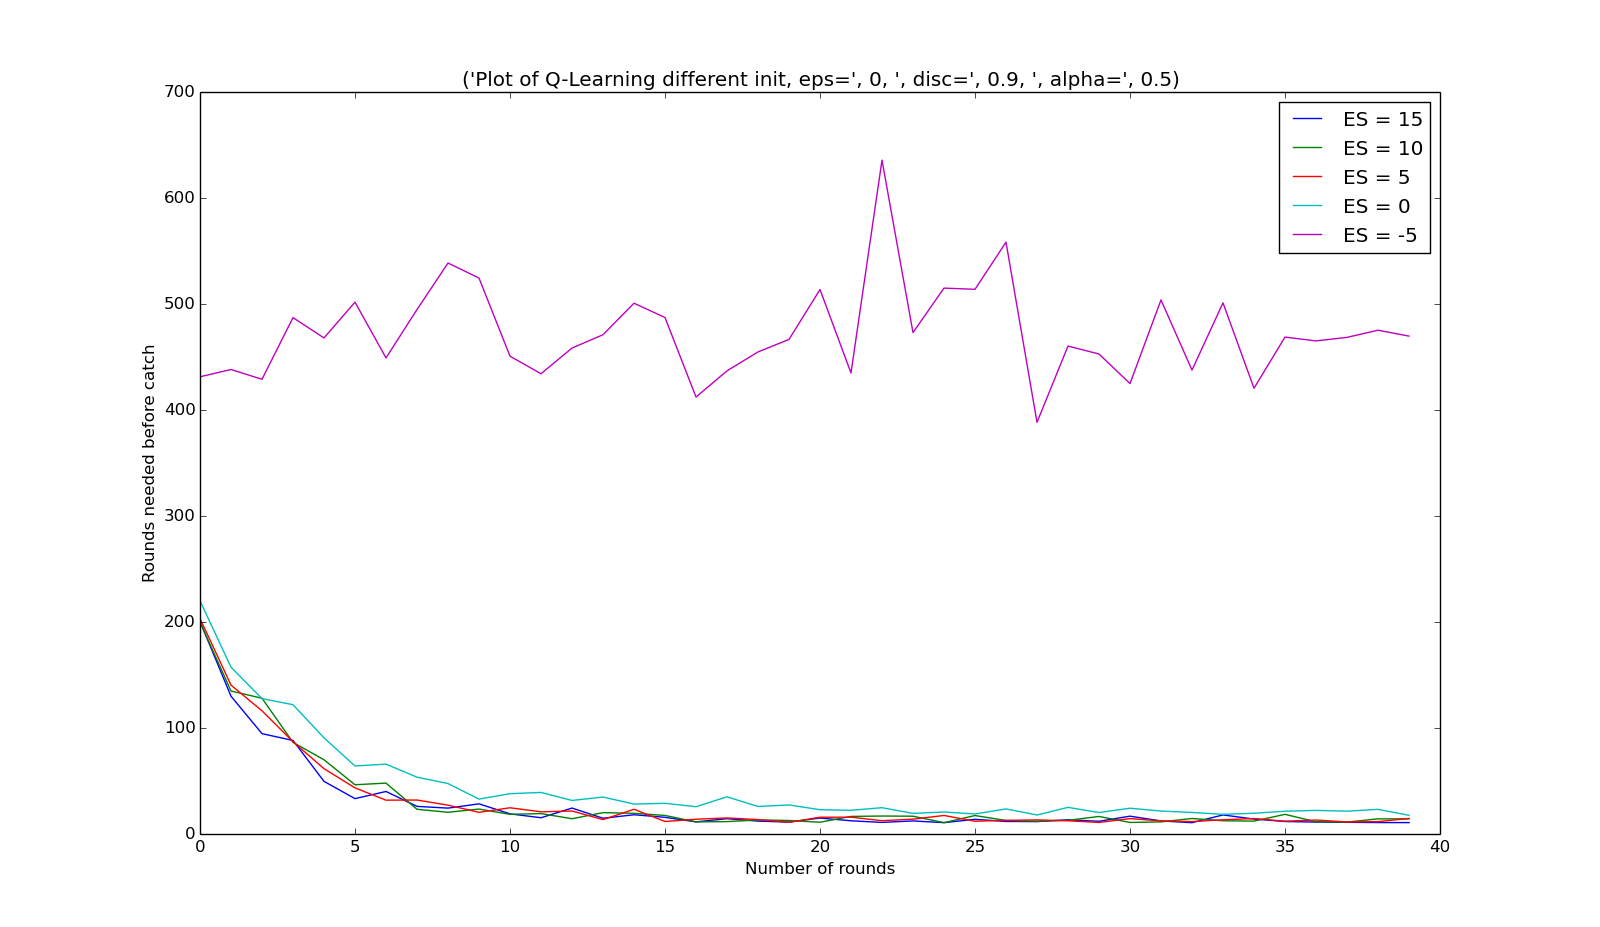
\includegraphics[scale=0.4]{q_learning_diff_init_epsilon_0}
%\caption{Q-learning with different initialization values and $\epsilon$ is 0}
%\end{center}
%\end{figure}

\section*{Conclusion}

\section*{Files attached}
\begin{itemize}
\item newstate.py
\item agents\_new.py
\item other\_objects.py
\item helpers.py \ldots
\end{itemize}
\section*{Sources}

\bibliography{bibliography}
\bibliographystyle{plain}
\begin{itemize}
	\item [1] Barto and Sutton (http://webdocs.cs.ualberta.ca/~sutton/book/the-book.html) \ldots
\end{itemize}

\end{document}
